\section{Casi d'uso}
\subsection{Scopo}
Lo scopo di questa sezione è la descrizione in elenco di tutti i casi d'uso individuati dal gruppo, in riferimento alle funzionalità dell'applicazione.
\subsection{Attori}
Come accordato con il proponente, non essendo richiesto alcun servizio di autenticazione attraverso un login o una registrazione, è presente un solo attore che può interagire con l'applicazione web:

\begin{figure}[h]
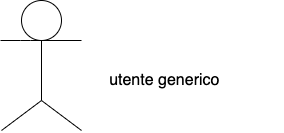
\includegraphics[width=1cm]{section/Images/Utente.png}
\centering
\caption{Gerarchia attori}
\end{figure}

\begin{description}
\item[Utente]:
Si riferisce all'utente utilizzatore che può accedere alla piattaforma.
\end{description}
Per un eventuale gestione di dati in più sessioni è quindi richiesta la funzionalità di poter salvare il proprio lavoro in un file scaricabile, che può poi essere successivamente caricato sulla piattaforma permettendo la ripresa del lavoro.
\subsection{Elenco casi d'uso}
\subsubsection{UC1 - Caricamento del dataset}
\begin{figure}[h]
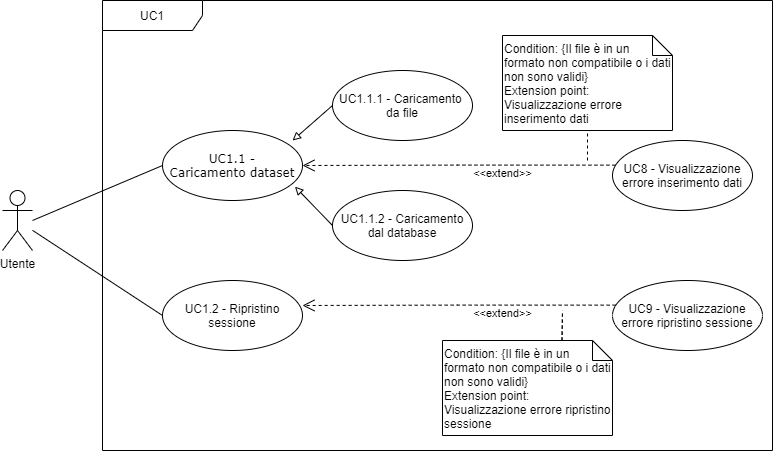
\includegraphics[width=\linewidth]{section/Images/UC1.png}
\centering
\caption{UC1 - Caricamento del dataset}
\end{figure}
\begin{itemize}
	\item \textbf{Attore primario}: Utente.
	\item \textbf{Precondizioni}: Il sistema è raggiungibile e funzionante.
	\item \textbf{Postcondizioni}: Viene visualizzato un messaggio che avvisa l'utente del corretto caricamento dei dati e della loro validità.
	\item \textbf{Scenario principale}:
		\begin{enumerate}
			\item L'utente accede al sistema;
			\item L'utente sceglie come ricavare i dati:
				\begin{enumerate}[(a)]
			\item L'utente seleziona la funzionalità "carica file" [UC1.1];
			\item L'utente seleziona un dataset tra quelli disponibili nel database [UC1.2].
				\end{enumerate}
		\end{enumerate}
	\item \textbf{Estensioni}:
	\begin{enumerate}[(a)]
		\item Nel caso in cui il file sia in un formato sbagliato o i dati non sono validi:
		\begin{enumerate}[1.]
			\item i dati non vengono caricati nel sistema;
			\item viene visualizzato un errore esplicativo [UC7].
		\end{enumerate}
	\end{enumerate}
\end{itemize}

\subsubsection{UC1.1 - Caricamento dataset da file}

\begin{itemize}
	\item \textbf{Attore primario}: Utente.
	\item \textbf{Precondizioni}: Il sistema è raggiungibile e funzionante. L'utente ha a disposizione un dataset in formato CSV.
	\item \textbf{Postcondizioni}: I dati presenti nel file vengono caricati nel sistema. Viene visualizzato un messaggio che avvisa l'utente del corretto caricamento e della validità dei dati.
	\item \textbf{Scenario principale}: L'utente sceglie di caricare un dataset personale o ricavato da altre fonti esterne.
	
\end{itemize}

\subsubsection{UC1.2 - Caricamento dataset dal database}

\begin{itemize}
	\item \textbf{Attore primario}: Utente.
	\item \textbf{Precondizioni}: Il sistema è raggiungibile e funzionante. L'utente effettua una query dal database disponibile per prelevare il dataset.
	\item \textbf{Postcondizioni}: I dati vengono caricati nel sistema. Viene visualizzato un messaggio che avvisa l'utente del corretto caricamento e della loro validità.
	\item \textbf{Scenario principale}: L'utente sceglie di caricare un dataset tra quelli presenti nel database.
	
\end{itemize}


  
\subsection{UC2 - Selezione delle dimensioni da utilizzare}
\begin{itemize}
	\item \textbf{Attore primario}: Utente;
	\item \textbf{Precondizioni}: L'utente ha caricato i dati nel sistema [UC1];
	\item \textbf{Postcondizioni}: Le dimensioni scelte vengono aggiornate nel sistema e i dati sono pronti per essere visualizzati [UC6];
	\item \textbf{Scenario principale}:
		\begin{enumerate}
			\item All'utente viene presentata una schermata con tutte le dimensioni presenti nel dataset caricato già selezionate di default;
			\item Per ogni dimensione è presente una cella da selezionare nel caso la si voglia utilizzare o meno;
			\item L'utente seleziona le dimensioni che desidera analizzare.
		\end{enumerate}
	\item \textbf{Estensioni:}
		\begin{enumerate}[(a)]
			\item Nel caso in cui l'utente non abbia selezionato nessuna dimensione:
			\begin{enumerate}[1.]
				\item Le dimensioni non vengono aggiornate nel sistema;
				\item Viene visualizzato un messaggio d'errore esplicativo [UC12].
			\end{enumerate}
		\end{enumerate}
\end{itemize}
\newpage
\subsubsection{UC3 - Scelta della \glo{visualizzazione}}
\begin{figure}[h]
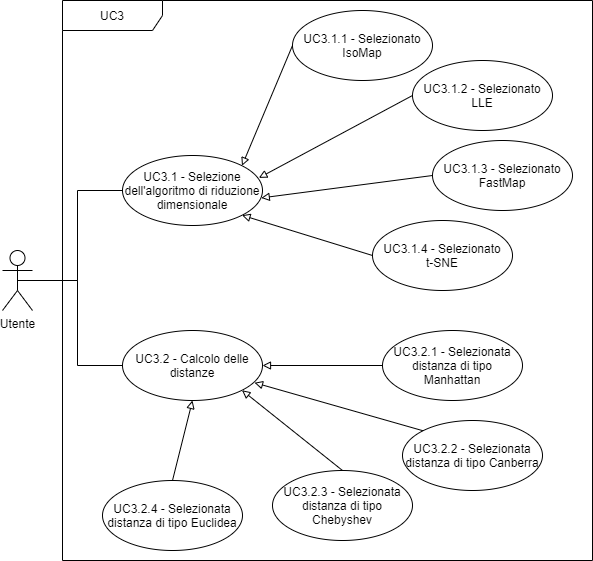
\includegraphics[width=\linewidth]{section/Images/UC3.png}
\centering
\caption{UC3 - Scelta della visualizzazione}
\end{figure}
\begin{itemize}
	\item \textbf{Attore primario}: Utente.
	\item \textbf{Precondizioni}: L'utente ha caricato dei dati nel sistema [UC1] e ha selezionato le dimensioni da utilizzare [UC2].
	\item \textbf{Postcondizioni}: Viene mostrata la visualizzazione scelta, con possibilità di personalizzazione [UC4].
	\item \textbf{Scenario principale}: L'utente seleziona una visualizzazione tra quelle disponibili.
	\item \textbf{Generalizzazioni}: L'utente seleziona una delle seguenti opzioni disponibili:
		\begin{enumerate}[(a)]
			\item \glo{\textit{Scatter Plot Matrix}} [UC3.1]
			\item \glo{\textit{Heat Map}} [UC3.2]
			\item \glo{\textit{Force Field}} [UC3.3]
			\item \glo{\textit{Proiezione Lineare Multi Asse}} [UC3.4]
		\end{enumerate}
	\item \textbf{Estensioni}:
	\begin{enumerate}[(a)]
		\item Nel caso in cui non è stato caricato alcun dato o non è stata scelta alcuna dimensione:
		\begin{enumerate}[1.]
			\item Il grafico non viene visualizzato;
			\item Viene visualizzato un errore esplicativo [UC9].
		\end{enumerate}
	\end{enumerate}
\end{itemize}
\subsubsection{UC3.1 - Scelta dell'algoritmo di riduzione dimensionale}
\begin{itemize}
	\item \textbf{Attore primario}: Utente;
	\item \textbf{Precondizioni}: L'utente ha caricato i dati e le dimensioni nel sistema [UC1];
	\item \textbf{Postcondizioni}: La scelta viene memorizzata nel sistema e viene resa disponibile una sezione per la personalizzazione dei parametri dell'algoritmo di riduzione dimensionale selezionato [UC4];
	\item \textbf{Scenario principale}: L'utente seleziona un algoritmo di riduzione dimensionale tra quelli resi disponibili dal sistema.
	\item \textbf{Generalizzazioni}: L'utente seleziona una delle seguenti opzioni:
	\begin{enumerate}[1.]
		\item \glo{\textit{Isometric Mapping (IsoMap)}} [UC3.1.1];
		\item \glo{\textit{Locally Linear Embedding (LLE)}} [UC3.1.2];
		\item \glo{\textit{Fast Mapping (FastMap)}} [UC3.1.3];
		\item \glo{\textit{T-distributed Stochastic Neighbor Embedding (t-SNE)}} [UC3.1.4].
	\end{enumerate}
\end{itemize}
\subsubsection{UC3.2 - Calcolo delle distanze}
\begin{itemize}
	\item \textbf{Attore primario}: Utente;
	\item \textbf{Precondizioni}: L'utente ha caricato i dati e le dimensioni nel sistema [UC1];
	\item \textbf{Postcondizioni}: La nuova dimensione viene salvata nel sistema e resa disponibili all'utente per procedere con la visualizzazione [UC5];

	\item \textbf{Scenario principale}: L'utente:
		\begin{enumerate}
			\item Seleziona tra le dimensioni disponibili (originarie e derivate da eventuali processi di riduzione dimensionale precedenti) quelle che saranno interessate dal processo di calcolo della distanza;
			\item Seleziona un tipo di distanza tra quelle a disposizione.
		\end{enumerate}			
	 
	
	\item \textbf{Generalizzazioni}: L'utente seleziona una delle seguenti opzioni:
	
	\begin{enumerate}[(a)]
		\item distanza di \glo{\textit{Manhattan}} [UC3.2.1];
		\item distanza di \glo{\textit{Canberra}} [UC3.2.2];
		\item distanza di \glo{\textit{Chebyshev}} [UC3.2.3].
	\end{enumerate}
\end{itemize}
\subsubsection{UC3.3 - Scelta visualizzazione Force Field}
\begin{itemize}
	\item \textbf{Attore primario}: Utente.
	\item \textbf{Precondizioni}: L'utente ha caricato dei dati nel sistema [UC1], ha selezionato le dimensioni da utilizzare [UC2] e ha scelto la visualizzazione \textit{Force Field} .
	\item \textbf{Postcondizioni}: Viene mostrata la visualizzazione \textit{Force Field}, con possibilità di modificare le dimensioni scelte.
	\item \textbf{Scenario principale}: L'utente seleziona la visualizzazione \textit{Force Field}
\end{itemize}
\subsubsection{UC3.4 - Scelta visualizzazione Proiezione Lineare Multi Asse}

\begin{itemize}
	\item \textbf{Attore primario}: Utente.
	\item \textbf{Precondizioni}: L'utente ha caricato dei dati nel sistema [UC1], ha selezionato le dimensioni da utilizzare [UC2] e ha scelto la visualizzazione \textit{Proiezione Lineare Multi Asse} .
	\item \textbf{Postcondizioni}: Viene mostrata la visualizzazione \textit{Proiezione Lineare Multi Asse}, con possibilità di personalizzazione del grafico [UC4.4].
	\item \textbf{Scenario principale}: L'utente seleziona la visualizzazione \textit{Proiezione Lineare Multi Asse} e il sistema ritorna un grafico con cui si può interagire.
\end{itemize}
\subsection{UC5 - Scelta della \glo{visualizzazione}}
\begin{figure}[h]
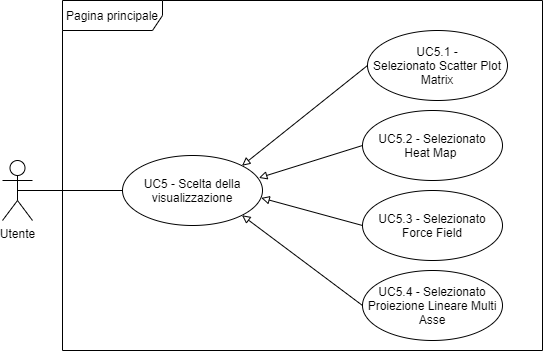
\includegraphics[width=\linewidth]{Section/Images/UC5.png}
\centering
\caption{UC5 - Scelta della visualizzazione}
\end{figure}
\begin{itemize}
	\item \textbf{Attore primario}: Utente;
	\item \textbf{Precondizioni}: L'utente ha caricato dei dati nel sistema e ha selezionato le dimensioni da utilizzare [UC2].
	\item \textbf{Postcondizioni}: Viene mostrata la visualizzazione scelta, con possibilità di personalizzazione [UC6]. La scelta viene salvata nel sistema.
	\item \textbf{Scenario principale}: L'utente seleziona la visualizzazione che vuole utilizzare tra quelle disponibili.
	\item \textbf{Generalizzazioni}: L'utente seleziona una delle seguenti opzioni:
		\begin{enumerate}
			\item \glo{\textit{Scatter Plot Matrix}} [UC5.1];
			\item \glo{\textit{Heat Map}} [UC5.2];
			\item \glo{\textit{Force Field}} [UC5.3];
			\item \glo{\textit{Proiezione Lineare Multi Asse}} [UC5.4].
		\end{enumerate}

\end{itemize}
\newpage
\subsection{UC6 - Personalizzazione della visualizzazione}
\begin{figure}[h]
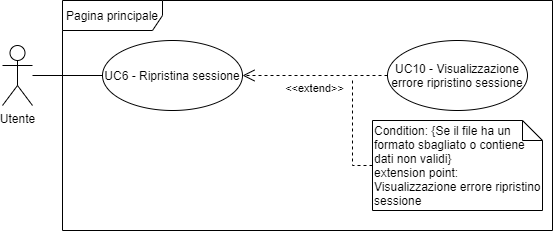
\includegraphics[width=\linewidth]{Section/Images/UC6.png}
\centering
\caption{Diagramma sulla personalizzazione della visualizzazione scelta}
\end{figure}
\begin{itemize}
	\item \textbf{Attore primario}: Utente;
	
	\item \textbf{Precondizioni}: L'utente ha scelto il grafico tra quelli a disposizione nel sistema [UC5];
	
	\item \textbf{Postcondizioni}: Il grafico viene aggiornato con le personalizzazioni impostate dall'utente;
	
	\item \textbf{Scenario principale}: L’utente sceglie come impostare le opzioni di personalizzazione del grafico. Verranno applicati, per ciascun campo, dei valori di default che l'utente può decidere di modificare o meno. In caso fosse stato precedentemente caricato un file di ripristino sessione [UC1.2] i valori di default iniziali diventerebbero quindi quelli specificati in questo file, lasciando comunque all'utente la possibilità di modificarli;
	
	\item \textbf{Generalizzazioni}: L'utente imposta i parametri di personalizzazione della visualizzazione scelta:
	\begin{enumerate}[(a)]
	\item Personalizzazione \textit{Scatter Plot Matrix} [UC6.1];
	\item Personalizzazione \textit{Adjacency Matrix} [UC6.2];
	\item Personalizzazione \textit{Force Field} [UC6.3];
	\item Personalizzazione \textit{Proiezione Lineare Multi Asse} [UC6.4];
	\item Personalizzazione \textit{Heat Map} [UC6.5].
	\end{enumerate}
		
\end{itemize}



\subsubsection{UC7 - Salva sessione}
\begin{itemize}
	\item \textbf{Attore primario}: Utente.
	\item \textbf{Precondizioni}: L'utente ha caricato dei dati nel sistema [UC1] e ha scelto il tipo di grafico da visualizzare [UC5]
	\item \textbf{Postcondizioni}: L'utente possiede un file \glo{JSON} per il ripristino della sessione.
	\item \textbf{Scenario principale}:
		\begin{enumerate}
			\item L'utente ha una sessione di lavoro aperta.
			\item L'utente seleziona la funzionalità "salva sessione";
			\item L'utente seleziona la directory in cui salvare il file.
		\end{enumerate}
\end{itemize}
\subsection{UC8 - Personalizzazione Force Field}
\begin{itemize}
	\item \textbf{Attore primario}: Utente.
	
	\item \textbf{Precondizioni}: L'utente ha scelto il grafico \textit{Force Field} [UC5.3].
	
	\item \textbf{Postcondizioni}: Il grafico viene aggiornato.
	
	\item \textbf{Scenario principale}: L'utente visualizza:
	
\begin{enumerate}
	\item Una lista con le funzioni di forza fornite dal sistema e può scegliere quale utilizzare tra quelle disponibili; 
	\item Una lista con tutte i tipi di distanza disponibili nel sistema e può scegliere quale utilizzare per il calcolo. 
\end{enumerate}	
	Inoltre l'utente può decidere alcuni stili del grafico, tra cui:
		\begin{enumerate}
			\item Scegliere quale dimensione utilizzare per il colore dei punti nel grafico;
				
			\item Scegliere quale dimensione utilizzare per la forma dei punti nel grafico;
			
			\item Scegliere quale dimensione utilizzare per l'etichetta dei punti nel grafico;
			
			\item Scegliere quale dimensione utilizzare per la dimensione dei punti nel grafico;
				
		\end{enumerate}
		
	\item \textbf{Estensioni}:
	\begin{enumerate}[(a)]
		\item ...
	\end{enumerate}
\end{itemize}


\subsubsection{UC9 - Personalizzazione Proiezione Lineare Multi Asse}
\begin{itemize}
	\item \textbf{Attore primario}: Utente.
	
	\item \textbf{Precondizioni}: L'utente ha scelto il grafico \textit{Proiezione Lineare Multi Asse} [UC5.4].
	
	\item \textbf{Postcondizioni}: Il grafico viene aggiornato.
	
	\item \textbf{Scenario principale}: L'utente sceglie che dimensioni visualizzare nel grafico tra quelle a disposizione. Inoltre può decidere alcune stili del grafico, tra cui:
		\begin{enumerate}
			\item Scegliere quale dimensione utilizzare per il colore dei punti nel grafico;
				
			\item Scegliere quale dimensione utilizzare per la forma dei punti nel grafico;
			
			\item Scegliere quale dimensione utilizzare per l'etichetta dei punti nel grafico;
			
			\item Scegliere quale dimensione utilizzare per la dimensione dei punti nel grafico;
				
		\end{enumerate}
		
	\item \textbf{Estensioni}:
	\begin{enumerate}[(a)]
		\item ...
	\end{enumerate}
\end{itemize}
\subsection{UC10 - Visualizzazione errore scelta dimensioni}
\begin{itemize}
	\item \textbf{Attore primario}: Utente;
	\item \textbf{Precondizioni}: L'utente non ha selezionato alcuna dimensione tra quelle presenti nel dataset precedentemente caricato;
	\item \textbf{Postcondizioni}: L'utente visualizza un messaggio di errore esplicativo;
	\item \textbf{Scenario principale}:
		\begin{enumerate}
			\item L'utente visualizza un messaggio di errore esplicativo;
			\item L'utente clicca "OK" per continuare.
		\end{enumerate}
\end{itemize}